\documentclass[11pt]{article}

\usepackage[a4paper,margin=1in]{geometry}
\usepackage[T1]{fontenc}
\usepackage[utf8]{inputenc}
\usepackage{lmodern}
\usepackage{microtype}
\usepackage{graphicx}
\usepackage{booktabs}
\usepackage{tabularx}
\usepackage{longtable}
\usepackage{array}
\usepackage{xcolor}
\usepackage{hyperref}
\usepackage{float}
\usepackage{enumitem}
\usepackage{titlesec}
\usepackage{caption}
\usepackage{subcaption}
\usepackage{fancyhdr}

\graphicspath{{../outputs/figures/}}

\definecolor{accent}{HTML}{1F3A5F}
\definecolor{warn}{HTML}{B0563A}
\definecolor{soft}{HTML}{F4F1EC}

\hypersetup{
  colorlinks=true,
  linkcolor=accent,
  urlcolor=accent,
  citecolor=accent,
  pdftitle={PCOS Pathfinder Technical Report},
  pdfauthor={Biohackathon 2026 Team},
  pdfsubject={Tiered clinical decision support for PCOS},
}

\setlist[itemize]{leftmargin=1.4em,topsep=2pt,itemsep=2pt}
\setlist[enumerate]{leftmargin=1.6em,topsep=2pt,itemsep=2pt}
\renewcommand{\arraystretch}{1.18}
\titleformat{\section}{\Large\bfseries\color{accent}}{\thesection}{0.6em}{}
\titleformat{\subsection}{\large\bfseries\color{accent!85!black}}{\thesubsection}{0.6em}{}
\captionsetup{font=small,labelfont=bf,labelsep=period}

\pagestyle{fancy}
\fancyhf{}
\renewcommand{\headrulewidth}{0pt}
\fancyfoot[L]{\small\color{accent}PCOS Pathfinder}
\fancyfoot[R]{\small\thepage}

\newcommand{\metric}[1]{\textbf{#1}}
\newcommand{\code}[1]{\texttt{\small #1}}

\title{\vspace{-1.5em}
\textcolor{accent}{\textbf{PCOS Pathfinder}}\\[0.4em]
\large A Tiered, Explainable Decision-Support Prototype\\
for Earlier PCOS Detection and Differential Diagnosis}
\author{Biohackathon 2026: Women's Health}
\date{11--22 May 2026}

\begin{document}
\maketitle
\thispagestyle{fancy}

\begin{abstract}
\noindent PCOS Pathfinder is a data-grounded clinical decision-support prototype for earlier identification of Polycystic Ovary Syndrome (PCOS) and broader differential workup in women's health. The system anchors on the required PCOS clinical dataset (n=541, Kerala, India), layers a synthetic endometriosis-overlap module for differential reasoning, and uses a lightweight single-cell gene-list check for biological rationale. The delivered artifacts are six reproducible notebooks, three saved scikit-learn models, a Streamlit clinician interface, exported metrics and figures, and this report. Thresholds are selected from out-of-fold training probabilities (no test leakage), risk tiers are anchored to each model's action threshold, and patient-level SHAP attributions are provided for both PCOS models. On the held-out test split the enhanced model reaches ROC-AUC 0.953 with recall 0.886 and specificity 0.902. The system is framed throughout as decision support, not standalone diagnosis.
\end{abstract}

\section{Challenge Context and Project Goal}

The Biohackathon 2026 challenge asks teams to improve diagnostic accuracy for women's health conditions using available data and a feasible implementation pathway. PCOS is the core case because it is common, heterogeneous, and frequently diagnosed late: clinicians must synthesise menstrual, metabolic, hormonal, ovarian, dermatologic, and reproductive information, and overlapping conditions are routinely missed.

A defensible solution therefore needs to do more than predict a binary label. It should help clinicians identify high-risk patients earlier, explain the drivers of risk in clinically familiar terms, and avoid tunnel vision when adjacent conditions share presentations. The project goal is to build \textbf{PCOS Pathfinder}, a clinician-facing tiered decision-support workflow with three linked components:

\begin{enumerate}
  \item \textbf{Frontline screening model}: a high-recall PCOS risk flag using symptoms and basic vitals only, intended for primary care, telehealth, and community clinics.
  \item \textbf{Enhanced diagnostic-support model}: a stronger model that uses laboratory and ultrasound features once further investigations are available.
  \item \textbf{Endometriosis-overlap prompt}: a synthetic-data workflow nudge that prompts broader differential workup when symptoms overlap. It is not a diagnostic claim.
\end{enumerate}

\section{Data Sources}

\begin{table}[H]
\centering
\caption{Dataset inventory}
\begin{tabularx}{\linewidth}{lrX}
\toprule
Dataset & Rows / samples & Use \\
\midrule
PCOS clinical (Kerala, India) & 541 patients & Required modelling foundation \\
Endometriosis (synthetic) & 10{,}000 rows & Differential-overlap prompt \\
PCOS single-cell archive & 20 samples & Biological rationale (gene-list peek) \\
Endometrium single-cell archive & 2 samples & Biological context only \\
\bottomrule
\end{tabularx}
\end{table}

The PCOS workbook's modelling sheet (\code{Full\_new}) contains 44 columns and a binary target \code{PCOS (Y/N)}. The class split is 364 non-PCOS to 177 PCOS, a roughly 2:1 imbalance.

\begin{figure}[H]
\centering
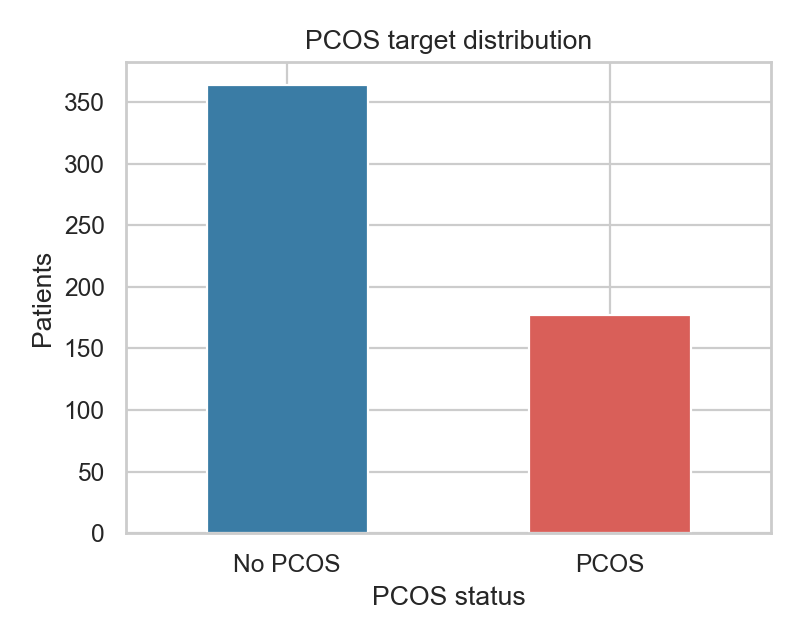
\includegraphics[width=0.55\linewidth]{pcos_class_balance.png}
\caption{PCOS class distribution in the required dataset.}
\end{figure}

The supplementary endometriosis dataset has seven variables: age, menstrual irregularity, chronic pain level, hormone-level abnormality, infertility, BMI, and diagnosis. Because it is synthetic, the resulting model is treated as a workflow prompt only. The single-cell archives are 10x-style outputs; this project deliberately limits itself to a gene-list peek rather than a full single-cell analysis, because the judging weights reward clinical usefulness over single-cell technique depth.

\section{Data Cleaning and Quality Controls}

Data cleaning is implemented in the notebook setup cells generated from \code{scripts/create\_training\_notebooks.mjs}. The key steps:

\begin{itemize}
  \item Load the \code{Full\_new} sheet; standardise names to lowercase snake case.
  \item Coerce every column with \code{pd.to\_numeric(errors="coerce")} and log every non-numeric cell to \code{outputs/metrics/pcos\_coercion\_report.csv}.
  \item Drop columns that cannot defensibly contribute:
  \begin{itemize}
    \item \code{sl\_no}, \code{patient\_file\_no} (identifiers).
    \item \code{blood\_group}: stored as ordinal codes 11--18, which has no meaningful order.
    \item \code{marriage\_status\_yrs}: clinically sensitive, not a diagnostic signal.
  \end{itemize}
  \item Engineer \code{cycle\_irregular\_flag} from \code{cycle\_r\_i} (Kaggle coding: 2 = regular, 4/5 = irregular).
  \item Cap visibly-impossible outliers in FSH, LH, FSH/LH, vitamin D3, and progesterone.
  \item Use median imputation \emph{inside} each scikit-learn pipeline, so imputation rules travel with the saved artifact.
\end{itemize}

\subsection{Data Caveat: ``Cycle Length'' Is Actually Bleeding Duration}

The source column labelled \code{Cycle length(days)} ranges 0--12 with a median of 5 across both classes -- this is the \emph{duration of menses bleeding in days}, not the menstrual cycle interval. The Kaggle dataset documentation is misleading on this point. The Streamlit prototype surfaces the field with the corrected label and a 0--12 range so clinicians do not accidentally enter a typical 28-day cycle value, which would be out-of-distribution and silently produce wrong predictions.

\subsection{Logged Coercions}

\begin{table}[H]
\centering
\caption{Non-numeric values silently coerced to missing during load}
\begin{tabular}{llc}
\toprule
Column & Example value & Count \\
\midrule
\code{ii\_beta\_hcg\_miu\_ml} & \code{1.99.} & 1 \\
\code{amh\_ng\_ml} & \code{a} & 1 \\
\bottomrule
\end{tabular}
\end{table}

\section{Model Design}

\subsection{Frontline Screening Model}

Intended for primary care, telehealth, and community settings. Lifestyle proxies (\code{fast\_food}, \code{reg\_exercise}) are intentionally excluded -- they are bias-prone, hard to validate at intake, and likely to encode confounders rather than physiology.

\begin{table}[H]
\centering
\caption{Screening feature set (13 features)}
\begin{tabularx}{\linewidth}{>{\raggedright\arraybackslash}X}
\toprule
Age, BMI, cycle pattern (raw and engineered flag), duration of menses bleeding, weight gain, hair growth, skin darkening, hair loss, pimples, random blood sugar, systolic blood pressure, diastolic blood pressure. \\
\bottomrule
\end{tabularx}
\end{table}

\subsection{Enhanced Diagnostic-Support Model}

Adds laboratory and ultrasound markers once further investigations are available.

\begin{table}[H]
\centering
\caption{Enhanced model additional features (14 added, 27 total)}
\begin{tabularx}{\linewidth}{>{\raggedright\arraybackslash}X}
\toprule
Haemoglobin, FSH, LH, FSH/LH ratio, TSH, AMH, prolactin, vitamin D3, progesterone, left and right follicle counts, left and right follicle sizes, endometrium thickness. \\
\bottomrule
\end{tabularx}
\end{table}

\subsection{Candidate Algorithms}

Both PCOS notebooks compare four models: a most-frequent dummy baseline, logistic regression with class-weight balancing and standard-scaling, a random forest with class-weight balancing, and gradient boosting. Selection is by 5-fold stratified cross-validation on the training split, ranking by ROC-AUC and breaking ties on recall. Across runs, random forest wins both contests.

\section{Validation Strategy}

A single stratified train/test split is used with \code{test\_size = 0.25} and \code{random\_state = 42}. Model selection uses 5-fold stratified cross-validation \emph{on the training split}. For each chosen model, action thresholds are selected using out-of-fold training probabilities from \code{cross\_val\_predict(method="predict\_proba")}. The threshold sweep targets recall $\geq 0.90$ on the training out-of-fold predictions while maximising specificity, then precision, then F1.

The held-out test set is then evaluated exactly once. This avoids the earlier risk of choosing a threshold on the test set and reporting optimistic metrics.

\section{Results}

\subsection{Held-Out Performance at the Chosen Thresholds}

\begin{table}[H]
\centering
\caption{Held-out test performance (n=136) at CV-selected high-recall thresholds}
\begin{tabular}{lrrrrrrr}
\toprule
Model & Threshold & ROC-AUC & Recall & Spec. & PPV & NPV & F2 \\
\midrule
Screening & 0.285 & 0.896 & 0.886 & 0.685 & 0.574 & 0.926 & 0.799 \\
Enhanced & 0.380 & 0.953 & 0.886 & 0.902 & 0.812 & 0.943 & 0.871 \\
Endometriosis (synth.) & 0.510 & 0.660 & 0.628 & 0.618 & 0.531 & --- & 0.609 \\
\bottomrule
\end{tabular}
\end{table}

The enhanced model improves specificity (0.685 $\to$ 0.902) and precision (0.574 $\to$ 0.812) while preserving the same recall as the screening model. NPV is 0.926 for screening and 0.943 for enhanced -- when either model says ``no PCOS'', it is right $>$92\% of the time, which is the right framing for ruling-out triage.

\subsection{Why F1 Is Not the Right Headline Metric for Screening}

The screening F1 of 0.696 is intentionally suppressed by the high-recall threshold. F1 weights precision and recall equally, but in primary-care screening the cost of a missed PCOS case (years of metabolic damage, infertility risk) is much larger than the cost of an over-referral (one additional clinical visit). Two more screening-aligned metrics behave very differently:

\begin{itemize}
  \item \textbf{Recall (0.886)} -- the screening tool catches 39 of the 44 PCOS-positive patients in the held-out cohort.
  \item \textbf{NPV (0.926)} -- when the tool says ``no PCOS'', the clinician can trust it.
  \item \textbf{F2 (0.799)} -- weights recall four times more than precision; this is the screening-friendly counterpart to F1.
\end{itemize}

Table~\ref{tab:tradeoff} compares the chosen high-recall threshold to a balanced 0.50 threshold for each model. The screening row makes the trade-off most visible: the balanced threshold raises F1 from 0.70 to 0.81 but loses four PCOS cases (recall 0.886 $\to$ 0.795). At the high-recall threshold, F2 is 0.80; at the balanced threshold, F2 is also 0.80 -- F2 is largely indifferent to the choice, so the high-recall threshold is the right pick under a sensitivity-first cost function.

\begin{table}[H]
\centering
\caption{Threshold trade-off on the held-out test set}
\label{tab:tradeoff}
\begin{tabular}{llrrrrrrr}
\toprule
Model & Threshold & Recall & Spec. & PPV & NPV & F1 & F2 & (TN, FP, FN, TP) \\
\midrule
\multirow{2}{*}{Screening} & 0.285 (chosen) & 0.886 & 0.685 & 0.574 & 0.926 & 0.696 & 0.799 & (63, 29, 5, 39) \\
                          & 0.500 (balanced) & 0.795 & 0.913 & 0.814 & 0.903 & 0.805 & 0.799 & (84, 8, 9, 35) \\
\midrule
\multirow{2}{*}{Enhanced} & 0.380 (chosen) & 0.886 & 0.902 & 0.812 & 0.943 & 0.848 & 0.871 & (83, 9, 5, 39) \\
                          & 0.500 (balanced) & 0.818 & 0.957 & 0.900 & 0.917 & 0.857 & 0.833 & (88, 4, 8, 36) \\
\bottomrule
\end{tabular}
\end{table}

For the enhanced model the high-recall threshold actually \emph{dominates} the balanced threshold under F2 (0.871 vs 0.833), so there is no headline F-score loss from the screening-friendly choice.

\subsection{ROC Curves and Confusion Matrices}

\begin{figure}[H]
\centering
\begin{subfigure}{0.48\linewidth}
  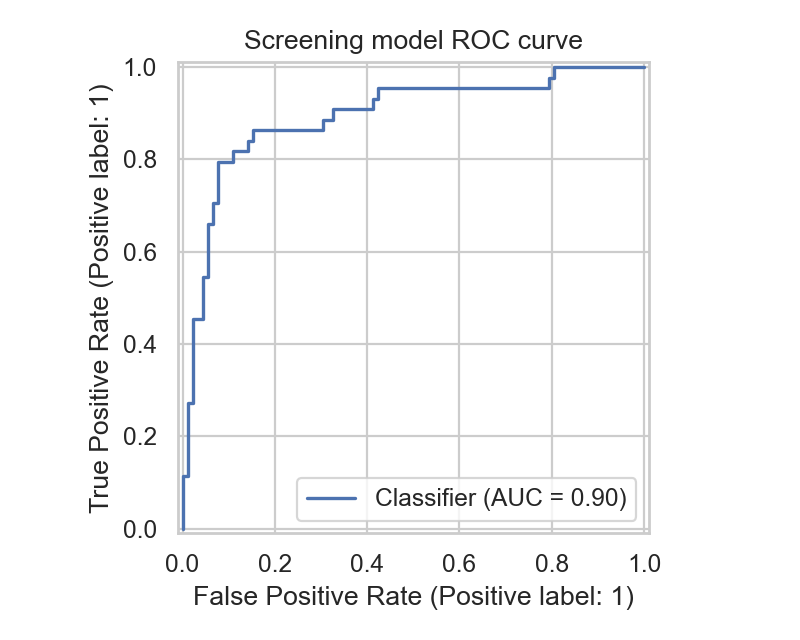
\includegraphics[width=\linewidth]{screening_roc_curve.png}
  \caption{Screening ROC, AUC = 0.896.}
\end{subfigure}\hfill
\begin{subfigure}{0.48\linewidth}
  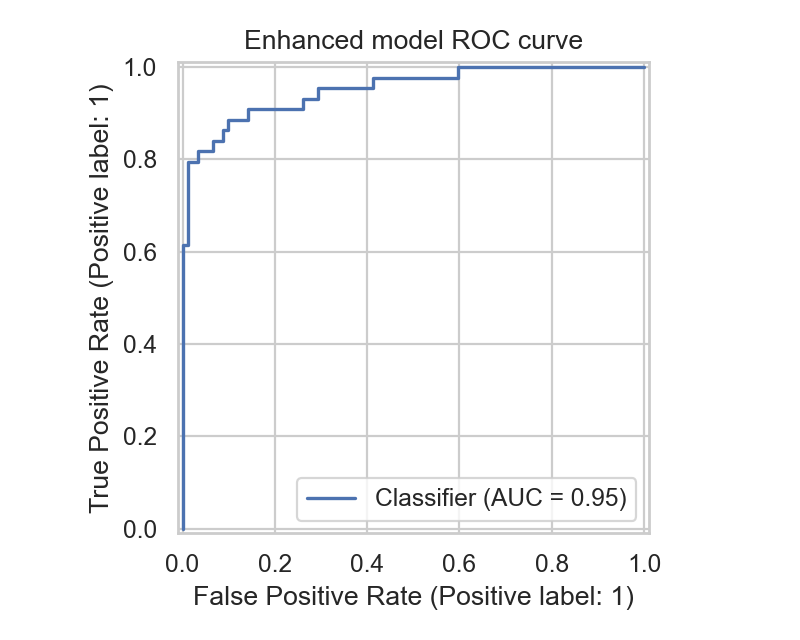
\includegraphics[width=\linewidth]{enhanced_roc_curve.png}
  \caption{Enhanced ROC, AUC = 0.953.}
\end{subfigure}
\caption{ROC curves on the held-out test set.}
\end{figure}

\begin{figure}[H]
\centering
\begin{subfigure}{0.48\linewidth}
  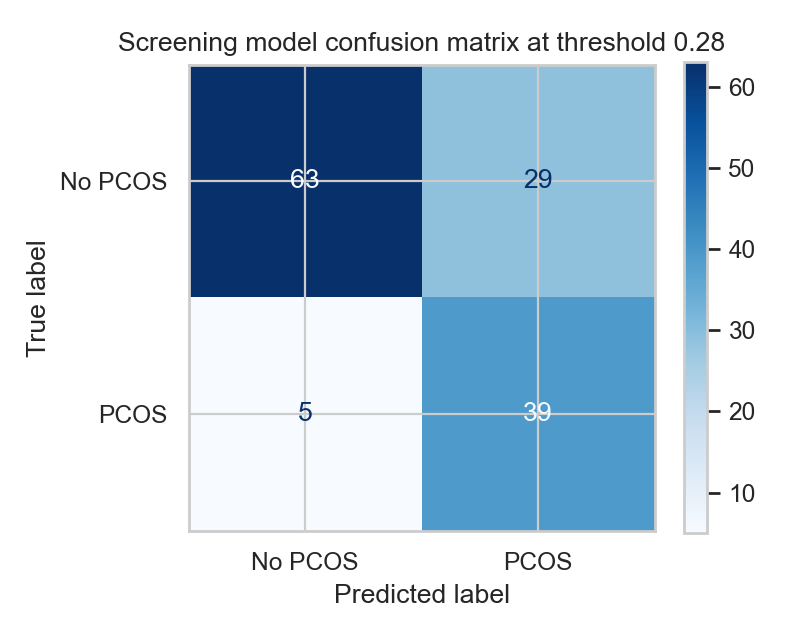
\includegraphics[width=\linewidth]{screening_confusion_matrix.png}
  \caption{Screening confusion at $t = 0.285$.}
\end{subfigure}\hfill
\begin{subfigure}{0.48\linewidth}
  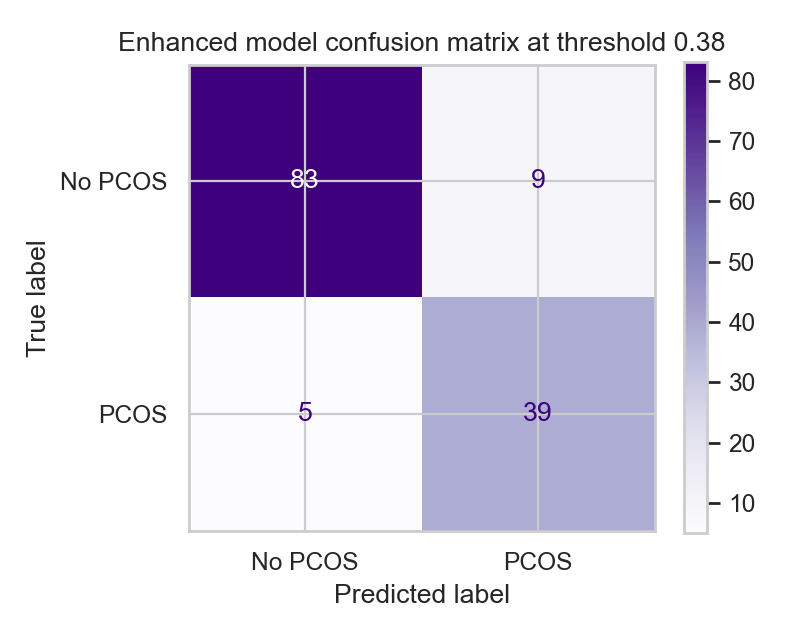
\includegraphics[width=\linewidth]{enhanced_confusion_matrix.png}
  \caption{Enhanced confusion at $t = 0.380$.}
\end{subfigure}
\caption{Confusion matrices at the CV-selected high-recall thresholds.}
\end{figure}

\section{Explainability}

Explainability is treated as a core product feature, not an afterthought.

\subsection{Global Drivers}

Global feature importances are exported per model. The screening model leans on symptom presentation (skin darkening, hair growth, weight gain) and basic vitals; the enhanced model is dominated by ultrasound (follicle counts) once those features are available.

\begin{figure}[H]
\centering
\begin{subfigure}{0.48\linewidth}
  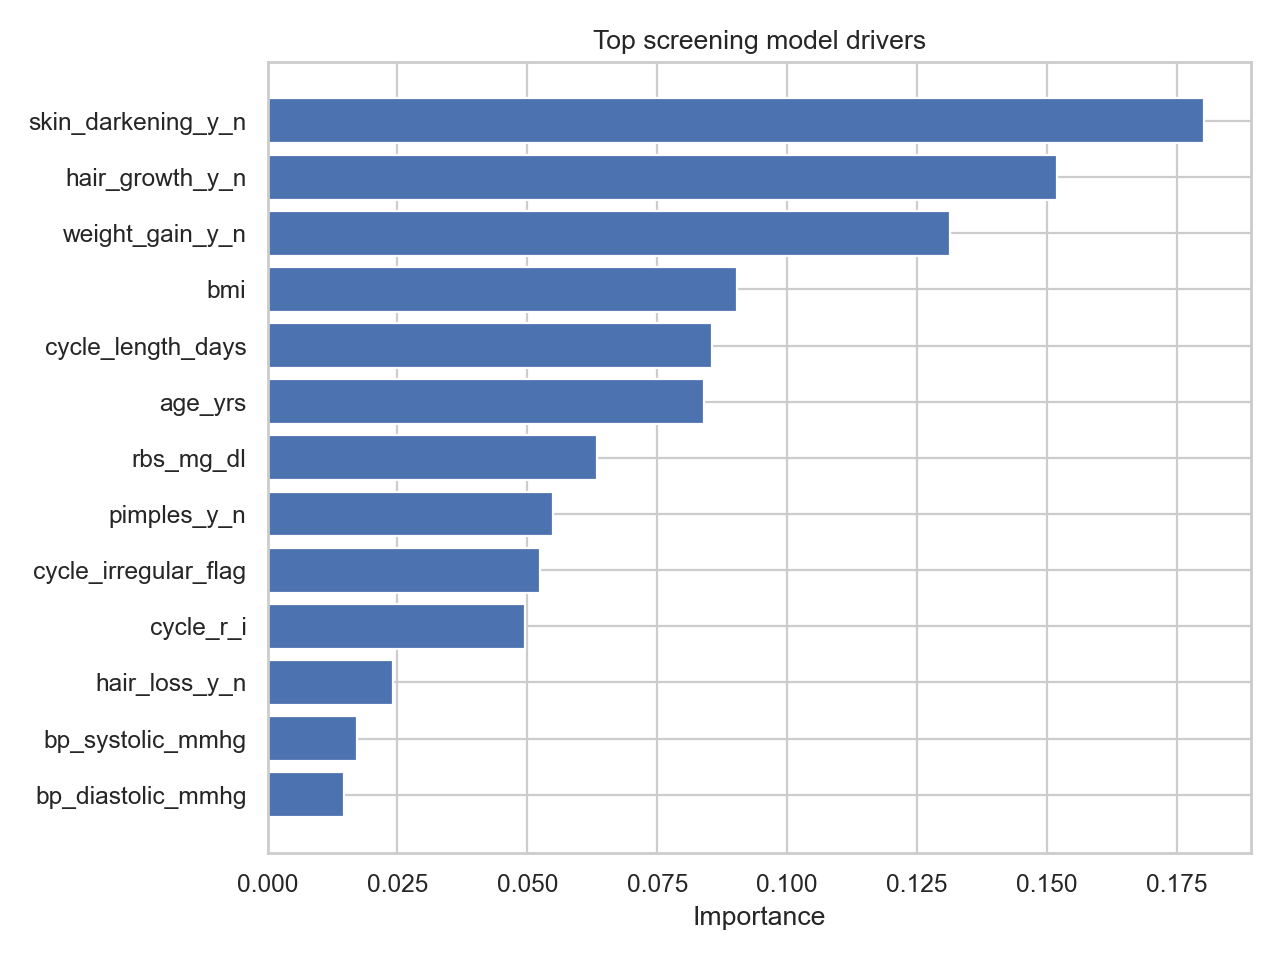
\includegraphics[width=\linewidth]{screening_feature_importance.png}
  \caption{Screening model.}
\end{subfigure}\hfill
\begin{subfigure}{0.48\linewidth}
  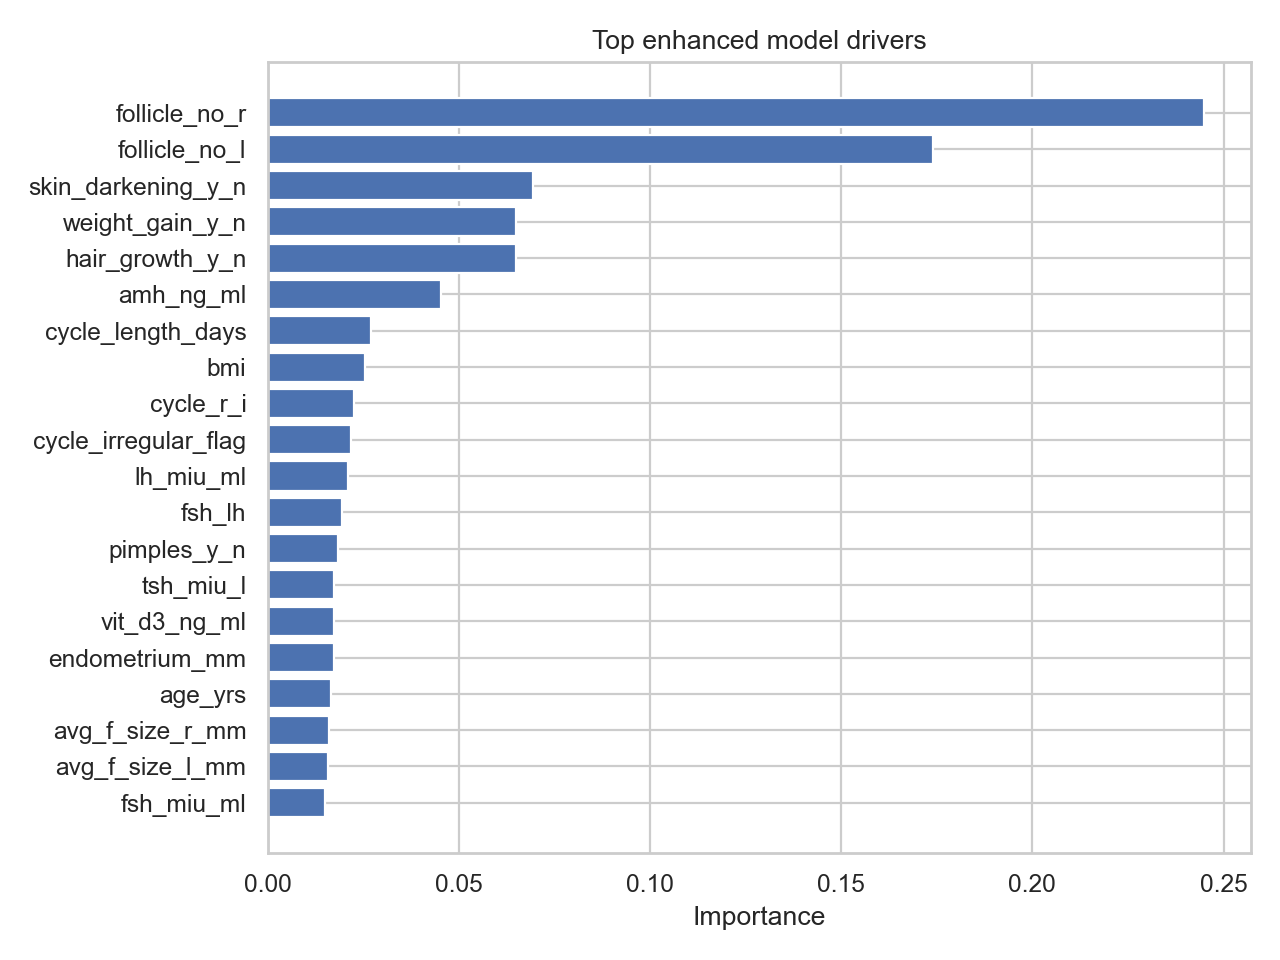
\includegraphics[width=\linewidth]{enhanced_feature_importance.png}
  \caption{Enhanced model.}
\end{subfigure}
\caption{Global feature importance.}
\end{figure}

\subsection{Patient-Level SHAP Attributions}

For tree models, \code{shap.TreeExplainer} produces fast and exact attributions. For logistic-regression fall-backs, each model artifact ships with a 100-row transformed training background that \code{shap.LinearExplainer} consumes. Demo cases are drawn from the held-out test slice (reproduced from the same random seed), so the explanations describe rows the model never saw during training.

\begin{figure}[H]
\centering
\begin{subfigure}{0.48\linewidth}
  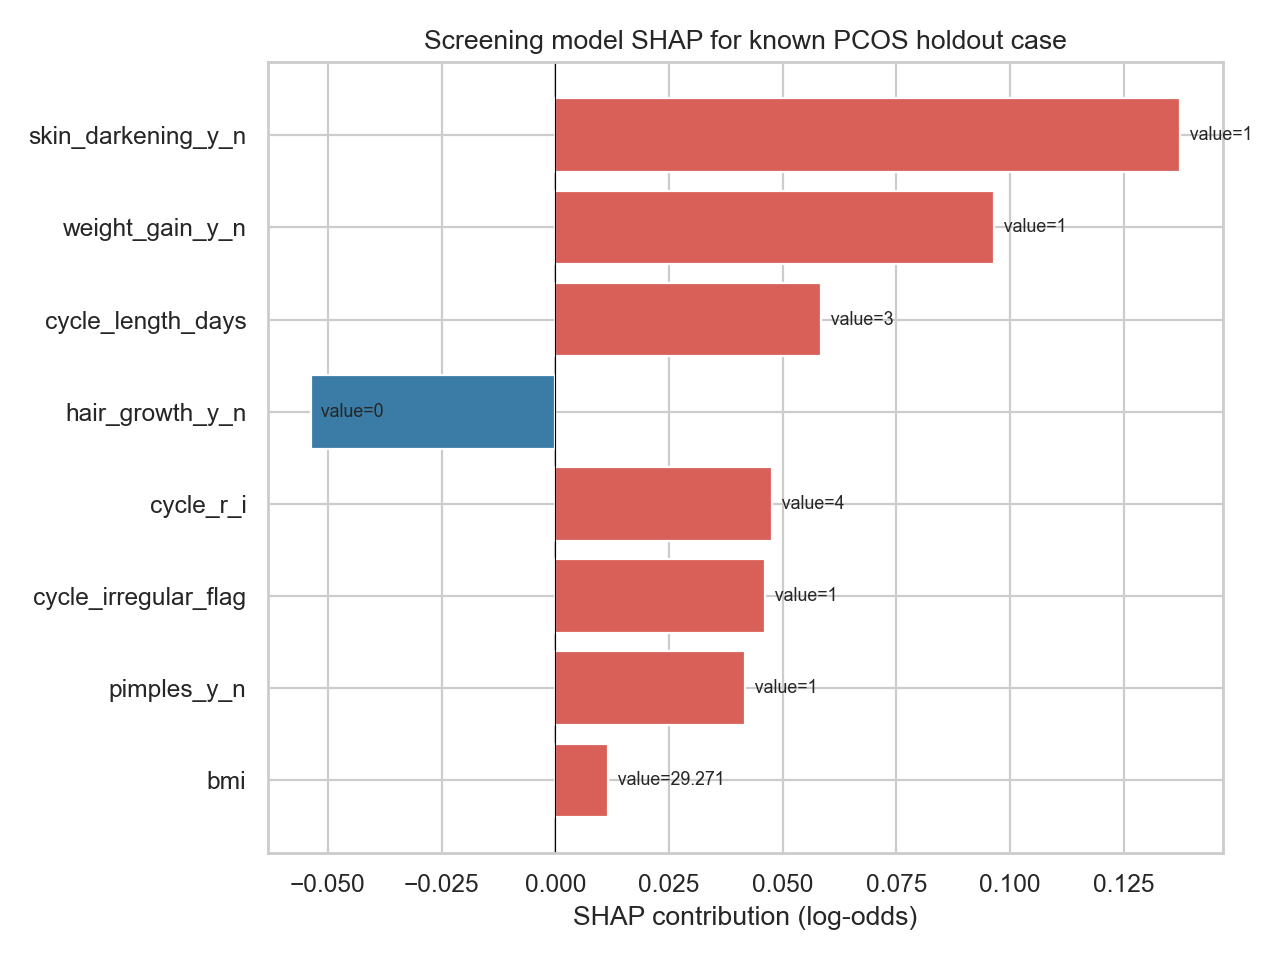
\includegraphics[width=\linewidth]{screening_shap_positive_case.png}
  \caption{Screening, positive holdout case.}
\end{subfigure}\hfill
\begin{subfigure}{0.48\linewidth}
  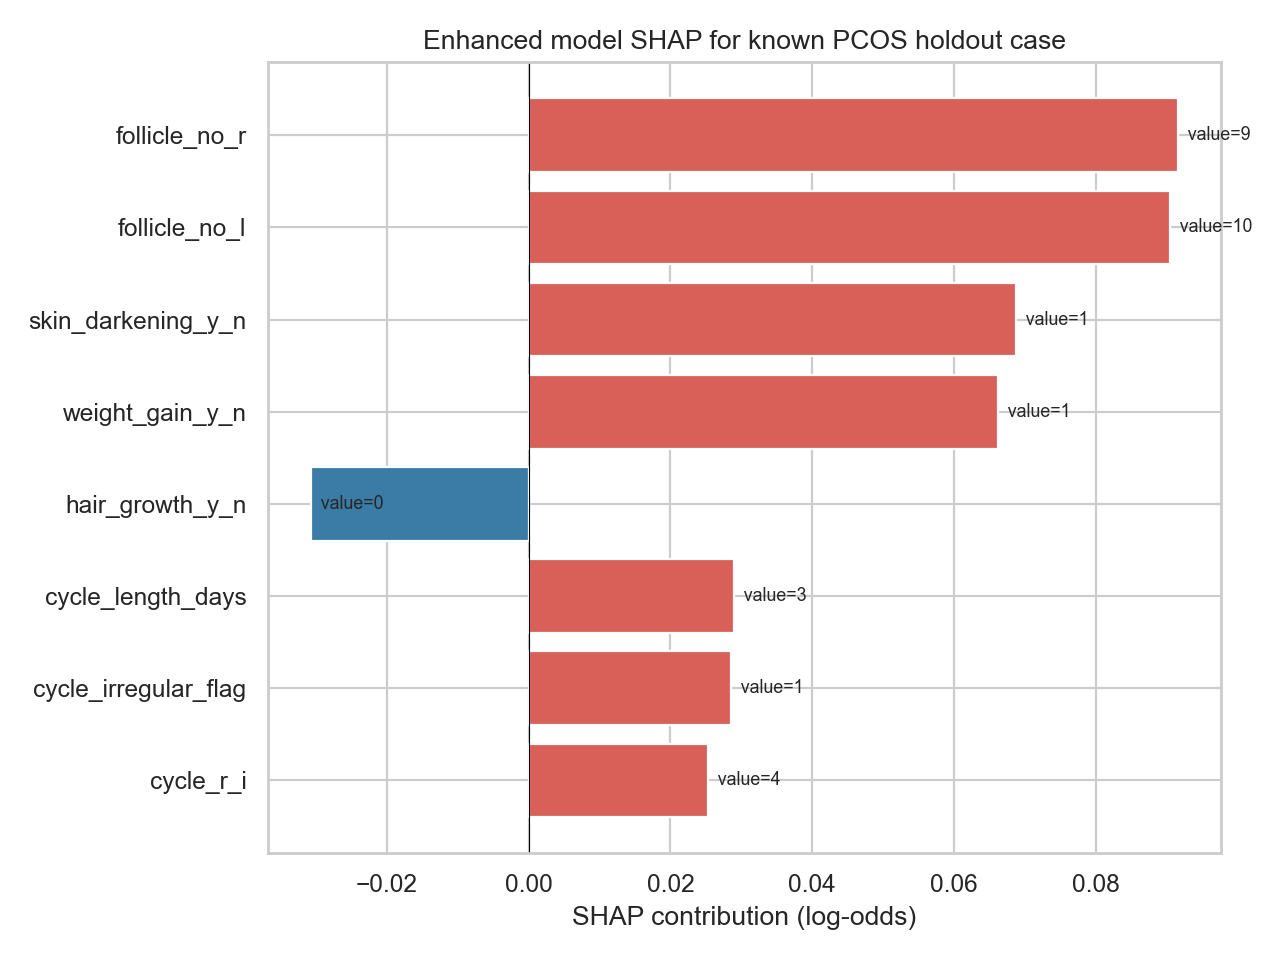
\includegraphics[width=\linewidth]{enhanced_shap_positive_case.png}
  \caption{Enhanced, positive holdout case.}
\end{subfigure}
\caption{SHAP log-odds contributions for one held-out PCOS-positive patient. Bars to the right increase PCOS probability.}
\end{figure}

\section{Differential-Diagnosis Prompt}

The endometriosis-overlap model is intentionally modest. It is trained on the supplementary synthetic dataset (10{,}000 rows) using six features (age, BMI, menstrual irregularity, chronic pain level, hormone-level abnormality, infertility) and reaches ROC-AUC 0.66 on a held-out split -- a level that reflects the limits of the underlying synthetic data rather than a modelling failure. In the prototype, a positive overlap score raises a warning that the clinician should consider a broader gynaecologic differential workup, especially when chronic pain and infertility are reported alongside menstrual irregularity. It is \emph{not} described as a validated endometriosis diagnostic model.

\section{Prototype}

The Streamlit prototype at \code{src/app.py} loads the three joblib model artifacts and presents three tabs:

\begin{itemize}
  \item \textbf{Patient assessment}: an intake form with collapsible sections for labs/ultrasound and differential-workup inputs, followed by stacked screening, enhanced, and endometriosis-overlap results. Each PCOS result shows probability, action threshold, threshold-anchored risk tier, and top SHAP drivers.
  \item \textbf{Population view}: symptom prevalence by PCOS status (source cohort, n=541) and headline model metrics.
  \item \textbf{About}: plain-language model descriptions, threshold strategy, and caveats.
\end{itemize}

Risk tiers are anchored to each model's threshold so the displayed tier never contradicts the action flag:

\begin{itemize}
  \item \textbf{Low}: probability below threshold.
  \item \textbf{Moderate}: probability from threshold to threshold + 0.20 (capped at 0.90).
  \item \textbf{High}: probability above the moderate band.
\end{itemize}

\section{Biological Rationale from Single-Cell Feature Lists}

Notebook 06 extracts feature symbols from one PCOS single-cell sample and checks for the presence of a curated list of literature-supported PCOS genes across steroidogenesis (CYP17A1, CYP19A1, HSD3B2, STAR), androgen signalling (AR, SRD5A1, SRD5A2, HSD17B3), follicular development (FSHR, LHCGR, GATA4), AMH signalling (AMH, AMHR2), insulin signalling (INSR, IRS1, IRS2, INS), and PCOS GWAS loci (DENND1A, THADA, FSHB). All 20 curated genes appear in the per-sample feature lists, giving the slide deck a defensible biological rationale for the clinical features the model uses. No QC, normalisation, integration, clustering, or differential expression analysis is claimed.

\section{Limitations and Risk Controls}

\begin{itemize}
  \item \textbf{Small, single-source PCOS dataset.} 541 patients from 10 hospitals in Kerala, India is not enough for deployment-level validation, and the geography may not generalise.
  \item \textbf{Synthetic endometriosis data.} The differential module is a workflow prompt, not a diagnostic claim.
  \item \textbf{Equity variables are unavailable.} Race, income, geography, and access-to-care measures are missing, so equity claims rest on workflow design and low-resource feasibility rather than measured outcome disparities.
  \item \textbf{Clinical framing.} All outputs are framed as risk, triage, and decision support, not diagnosis.
  \item \textbf{Version sensitivity.} scikit-learn model artifacts are sensitive to version skew; \code{requirements.txt} pins the exact versions used during training.
  \item \textbf{Threshold philosophy.} Tiered thresholds favour sensitivity; clinicians who prefer specificity-first triage can switch to the balanced threshold reported in Table~\ref{tab:tradeoff} without retraining.
\end{itemize}

\section{Reproducible Artifacts}

\begin{longtable}{p{0.34\linewidth}p{0.58\linewidth}}
\toprule
Artifact & Purpose \\
\midrule
\code{notebooks/01\_pcos\_data\_audit\_and\_eda.ipynb} & Data loading, cleaning, audit, EDA, processed CSV export. \\
\code{notebooks/02\_train\_pcos\_screening\_model.ipynb} & Training, threshold selection, and evaluation of the screening model. \\
\code{notebooks/03\_train\_pcos\_enhanced\_model.ipynb} & Training and evaluation of the enhanced labs/ultrasound model. \\
\code{notebooks/04\_train\_endometriosis\_overlap\_model.ipynb} & Synthetic-data differential prompt model. \\
\code{notebooks/05\_thresholds\_explainability\_and\_demo.ipynb} & SHAP attributions, held-out demo cases, model card. \\
\code{notebooks/06\_single\_cell\_gene\_peek.ipynb} & Lightweight biological-rationale gene-list check. \\
\code{src/app.py} & Streamlit clinician-facing prototype. \\
\code{outputs/models/*.joblib} & Saved model artifacts (with SHAP backgrounds). \\
\code{outputs/metrics/*} & Held-out metrics, threshold trade-offs, SHAP tables, model card, audit reports. \\
\code{scripts/create\_training\_notebooks.mjs} & Deterministic notebook regenerator (the source of truth). \\
\code{report/build\_pdf.py} & Reportlab generator for this PDF. \\
\code{PROJECT\_PLAN.md, README.md, SUBMISSION.md} & Plan, quickstart, packaging checklist. \\
\bottomrule
\end{longtable}

\section{Conclusion}

The defensible pitch for PCOS Pathfinder is not automated diagnosis. It is a practical, explainable, tiered workflow that helps clinicians identify high-risk patients earlier (recall $\geq 0.88$), choose appropriate next investigations (the enhanced model dominates F2 at the same recall), and avoid overlooking adjacent women's health conditions (the differential prompt). The cleaning rules, threshold strategy, and SHAP attributions are reproducible end-to-end from the six numbered notebooks; the Streamlit prototype loads the same artifacts a clinician would use; and the limitations are stated up-front in the model card.

\end{document}
